%%%%%%%%%%%%%%%%%%%%%%%%%%%%%%%%%%%%%%%%%
% Journal Article
% LaTeX Template
% Version 1.4 (15/5/16)
%
% This template has been downloaded from:
% http://www.LaTeXTemplates.com
%
% Original author:
% Frits Wenneker (http://www.howtotex.com) with extensive modifications by
% Vel (vel@LaTeXTemplates.com)
%
% License:
% CC BY-NC-SA 3.0 (http://creativecommons.org/licenses/by-nc-sa/3.0/)
%
%%%%%%%%%%%%%%%%%%%%%%%%%%%%%%%%%%%%%%%%%

%----------------------------------------------------------------------------------------
%	PACKAGES AND OTHER DOCUMENT CONFIGURATIONS
%----------------------------------------------------------------------------------------

\documentclass[twoside,twocolumn]{article}

\usepackage{blindtext} % Package to generate dummy text throughout this template 

\usepackage[sc]{mathpazo} % Use the Palatino font
\usepackage[T1]{fontenc} % Use 8-bit encoding that has 256 glyphs
\linespread{1.05} % Line spacing - Palatino needs more space between lines
\usepackage{microtype} % Slightly tweak font spacing for aesthetics

\usepackage[english]{babel} % Language hyphenation and typographical rules

\usepackage[hmarginratio=1:1,top=32mm,columnsep=20pt,left=2cm,right=2cm,top=2cm,bottom=2cm]{geometry} % Document margins
\usepackage[hang, small,labelfont=bf,up,textfont=it,up]{caption} % Custom captions under/above floats in tables or figures
\usepackage{booktabs} % Horizontal rules in tables

\usepackage{lettrine} % The lettrine is the first enlarged letter at the beginning of the text

\usepackage{enumitem} % Customized lists
\setlist[itemize]{noitemsep} % Make itemize lists more compact

\usepackage{abstract} % Allows abstract customization
\renewcommand{\abstractnamefont}{\normalfont\bfseries} % Set the "Abstract" text to bold
\renewcommand{\abstracttextfont}{\normalfont\small\itshape} % Set the abstract itself to small italic text

\usepackage{titlesec} % Allows customization of titles
\renewcommand\thesection{\Roman{section}} % Roman numerals for the sections
\renewcommand\thesubsection{\roman{subsection}} % roman numerals for subsections
\titleformat{\section}[block]{\large\scshape\centering}{\thesection.}{1em}{} % Change the look of the section titles
\titleformat{\subsection}[block]{\large}{\thesubsection.}{1em}{} % Change the look of the section titles

\usepackage{fancyhdr} % Headers and footers
\pagestyle{fancy} % All pages have headers and footers
\fancyhead{} % Blank out the default header
\fancyfoot{} % Blank out the default footer
\fancyhead[C]{Running title $\bullet$ May 2016 $\bullet$ Vol. XXI, No. 1} % Custom header text
\fancyfoot[RO,LE]{\thepage} % Custom footer text

\usepackage{titling} % Customizing the title section

\usepackage{hyperref} % For hyperlinks in the PDF

% Packages maison
\usepackage{amsmath,amssymb} % For including math equations, theorems, symbols, etc
\usepackage{mathtools}
\usepackage{bm}
\usepackage{graphicx} % Required for including images
\graphicspath{{../Figures/}} % Set the default folder for images
\usepackage{prettyref}

%----------------------------------------------------------------------------------------
%	TITLE SECTION
%----------------------------------------------------------------------------------------

\setlength{\droptitle}{-4\baselineskip} % Move the title up

\pretitle{\begin{center}\Huge\bfseries} % Article title formatting
\posttitle{\end{center}} % Article title closing formatting
\title{A database linking piano and orchestral MIDI scores for automatic projective orchestration \textbf{(RESTREINT LE CHAMP D'APPLICATION, C'EST DOMMAGE NON ?)}} % Article title
\author{%
\textsc{L\'eopold Crestel, Philippe Esling}\\[1ex] % Your name
\normalsize IRCAM \\ % Your institution
\normalsize \href{mailto:leopold.crestel@ircam.fr}{leopold.crestel@ircam.fr} % Your email address
%\and % Uncomment if 2 authors are required, duplicate these 4 lines if more
%\textsc{Jane Smith}\thanks{Corresponding author} \\[1ex] % Second author's name
%\normalsize University of Utah \\ % Second author's institution
%\normalsize \href{mailto:jane@smith.com}{jane@smith.com} % Second author's email address
}
\date{\today} % Leave empty to omit a date
\renewcommand{\maketitlehookd}{%
\begin{abstract}
\noindent This article introduces the Projective Orchestral Database \textbf{POD}, a freely-available collection of midi scores composed of pairs linking piano scores to their corresponding orchestrations. To our best knowledge, this is the first database of its kind. 
This can allow to perform piano or orchestral prediction, but more importantly to try to learn the correlation between piano and orchestral scores.
Hence, we introduce the projective orchestration task, which consists in learning to perform automatic orchestration of a piano score. 
This task can be seen as the generation of a symbolic time series (an orchestral score) conditioned by another symbolic time series (the piano score).
We show how this task can be addressed using learning methods and also provide methodological guidelines to use the database.
\end{abstract}
}

%----------------------------------------------------------------------------------------

\begin{document}

% Print the title
\maketitle

%----------------------------------------------------------------------------------------
%	ARTICLE CONTENTS
%----------------------------------------------------------------------------------------

\section{Introduction}
% Orchestration = definition
Orchestration is the subtle art of writing musical pieces for the orchestra by combining the properties of various instruments in order to achieve a particular sonic rendering. \cite{koechli_orch,Rimsky-Korsakov:1873aa}. 
% Orchestration projective
Among the different writing techniques for orchestration, we define \textit{projective orchestration} as the technique which consists in writing first a piano score and then projecting it on an orchestra (\prettyref{fig:orch}). This technique has been long used by classic composers.
See for instance \textit{Pictures at an exhibition} written by Modest Mussorgsky and orchestrated by Maurice Ravel.
% Dataset symbolic pour l'orchestration projective
This paper introduces what is to our best knowledge, the first symbolic dataset of projective orchestrations.
% Rapide description
It contains pairs of a piano piece and an associated orchestration written by famous composers. Note that several orchestrations can be found for one given piano score.
This database has several purposes :
\begin{itemize}
	\item being the starting point for a scientific investigation of orchestration, especially for statistic-based approaches on high-level symbolic information
	\item establishing a reference dataset for the evaluation of generative algorithms 
	\item indexing works of famous composers for musicological purposes
\end{itemize}

The remainder of this paper is organized as follows. The first section details the structure of the database. An automatic projective orchestration task is introduced in section two, along with an evaluation framework and several proposition of learning based models that rely on the database.  Conclusions are provided in the last section.

\section{Dataset}
\subsection{A scientific investigation of orchestration}
% Teaching orchestration = exemples
Several treatises have been written by famous composers in an attempt to formalize orchestration (\cite{koechli_orch,piston-orch,Rimsky-Korsakov:1873aa}).
They compound a remarkable sum of examples, but do not build a comprehensive theorization.
% Why ? Because it is highly complex, and we can't handle this complexity
An explanation of this observation lies in the tremendous complexity that emerges from an orchestral work. The number of pitch and intensity ranges of each instrument is powered by the number of instruments in the orchestra, and lead to a huge combinatoric. During the performance, acoustic summation of the instruments give rise to highly non-linear effects at the signal level, which make the resulting sound almost impossible to predict. Eventually, only a little is known about the complex psycho-acoustic phenomena involved in the listening process.
It seems almost impossible for a human mind to grasp in its entirety the intertwined mechanisms of an orchestral rendering.

%% SYMBOLIC
% Problem too complex : need for scientific investigation
Hence, we believe that a thorough scientific investigation could help disentangling the multiple factors involved in an orchestral work, and might be a precious help toward a greater understanding of the discipline.
% Scientific investigation already made ? Yes : signal et psycho-ac
If major works have already been produced in psycho-acoustic \cite{mcadams2013timbre,pressnitzer2000perception,tardieu2012perception} and signal processing \cite{peeters2011timbre}, no attempts have been made to tackle orchestration from a symbolic perspective (i.e. considering score instead of audio signal).
% Utilité du symboliques
However, symbolic representations convey high-level information about the intuitive knowledge composers have about timbre manipulations. 
% Pourquoi c'est intéressant les orchestrations projectives ?
Especially through projective orchestration (\prettyref{fig:orch}), because it allows to observe how a composer highlights the existing harmonic, rhythmic and melodic structure of a piano piece with a timbral structure.

% Pourquoi pas de symbolique alors ? Complexité + pas encore les techniques adaptées
From a computational point of view, symbolic data involve an important complexity.
The average pitch range of an instrument powered by the number of instruments is a rough approximation of the large combinatoric engendered by a symphonic orchestra. Even for a computer, an exhaustive investigation of all the possible combinations is unimaginable.
% Et maintenant on a le deep learning
But the recent advents in machine learning brought techniques that could cope with the dimensionality involved by symbolic data.
% Mais on a besoin de... DATA :)
Based on statistical tools, those techniques require a huge amount of data. Unfortunately, there is no free-access symbolic database for orchestration.
This dataset is a first attempt to fill this gap by building a freely accessible symbolic database of projective orchestrations.

\begin{figure}
\centering
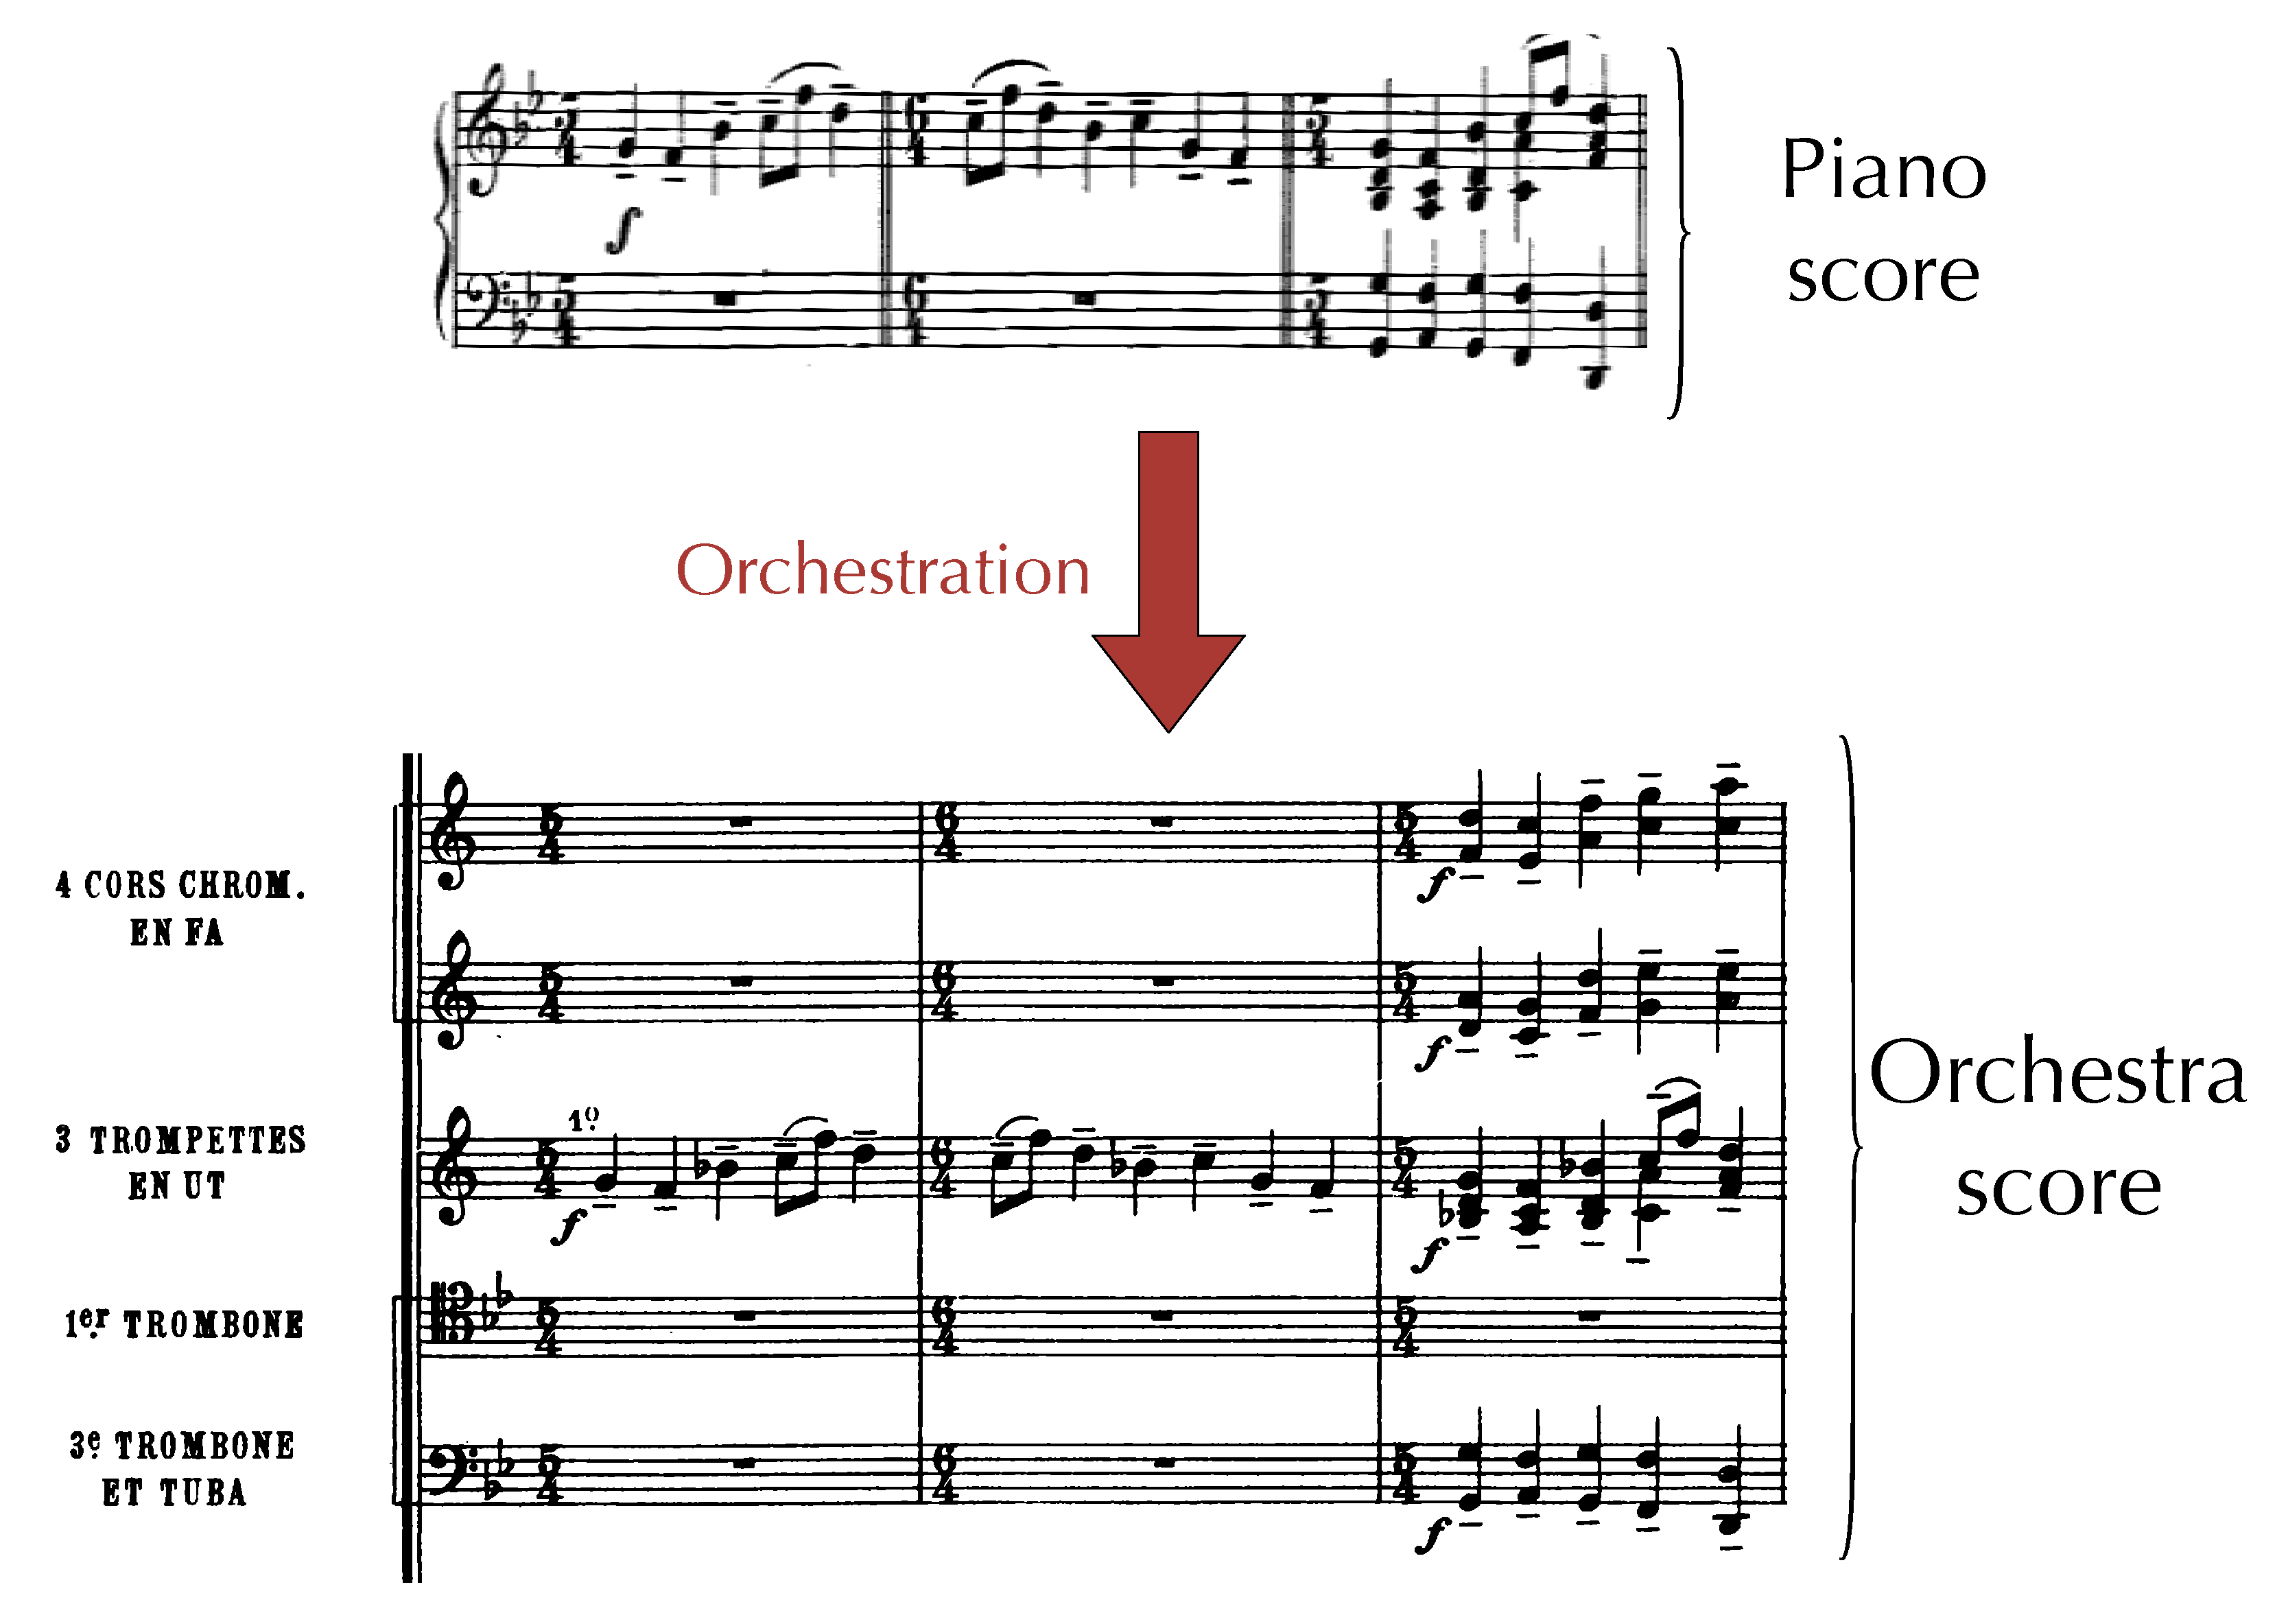
\includegraphics[scale=0.14]{Data_representation/orch}
\caption{\textit{Projective orchestration}. A piano score is projected on an orchestra. Even though a wide range of orchestrations exist for a given piano score, all of them will share strong relations with the original piano score. One given orchestration implicitly embeds the knowledge of the composer about timbre and orchestration.}
\label{fig:orch}
\end{figure}

\subsection{Structure of the database}
\paragraph{Organization}
% Number of file, main aspect a+ Format midi
The \textbf{POD} database contains piano and orchestra scores in the MIDI format.
% Organization, hierarchy
Those files are grouped by pair of a piano score and an orchestral version of it. Orchestration have been written by famous composers \textbf{VBOULIANE ???}.
Each pair is stored in a folder indexed by a number.
% Where does it come from
The files have been manually collected on several free-access databases found on the Internet (\textbf{CITE ??}).

\paragraph{Instrumentation}
% CSV instrumentation
The files gathered in the database have various origins. Then, one given instrument names can be found under a variety of aliases and abbreviations. 
In most of the orchestral midi files, each track is associated to one instrument, and the instrumentation is given by the names of the midi tracks.
Hence, a comma separated value (\textit{CSV}) file is associated to each \textit{MIDI} file. It has the same name as the midi file and only the extension is modified. It links the name of the midi tracks to the name of an instrument.

\paragraph{Metadata}
% Metadata
At the root of the database folder, a \textit{metadata.csv} file can be found. It gathers, for each folder index, the relative path to the folder from the database root directory, and when available, the composer and song name for the orchestral and piano works.
% Other statistics
\textbf{General statistics about the whole database can be found in the \textit{statistics.txt} file : the number of composers, the number of instruments} \textbf{USELESS ??}.

\paragraph{Integrity}
% Manually checked
Both metadata and instrumentation csv files have been automatically generated, but manually checked. We adopted a conservative approach when sorting the files. For instance, we automatically rejected a file with the slightest ambiguity between a midi track name and a possible instrument (for instance \textit{bass} can refer to \textit{double-bass} or \textit{voice bass}).

\paragraph{Score alignement}
% Aligned and non-aligned versions
Two versions of the database can be downloaded. The first version contains unmodified midi files as they were originally found on the diverse websites. The second version contains midi files automatically aligned using a \textit{Needleman-Wunsch} \cite{NEEDLEMAN1970443} based  algorithm detailed in the next section (\prettyref{:automatic-alignment}).

\paragraph{Formats}
% Matrices
Eventually, we offer the possibility to download a piano-roll (\prettyref{fig:piano-roll}) version of the database. In this case, all the midi files of piano (respectively orchestra) work have been transformed and concatenated into a unique two dimensional matrix. The starting and ending time of each track is indicated in the \textit{metadata.csv} file. \textbf{Those matrices (one for the piano, one for the orchestra) can be downloaded as \textit{.mat} (Matlab) or pickle (Python) files OR JUST CSV ????}

\subsection{Construction of the database}
% Automatic search for projective orchestration match
\paragraph{Automatic search for pairs}
A gigantic number of \textit{MIDI} files can be found on the Internet.
Although it seems that a lot of piano and orchestra pairs can be found among these databases,
finding them is a tedious task. Indeed, neither the organisation nor the meta-data have been thought for the purpose of projective orchestration.
 Hence, we tried to form pairs by finding similar file names and music keys, and used the instrumentation to ensure that we have on one side a score for solo instrument, and an orchestral on the other side. 
For matching file names, a fuzzy string matching algorithm based on the \textit{Levenshtein} distance (\cite{fuzzywuzzy}).

% Automatic alignment
\paragraph{Automatic alignment}
% Constat : toutes les partitions ne sont pas alignées
\label{:automatic-alignment}
Given the diverse origins of the midi files, it often happens that a piano score and its proposed orchestration were not aligned. Indeed, one file can be shorter than the other one, because of a dilation factor or skipped parts.
% A quoi ça sert d'avoir des partitions alignées ?
Those misalignments were problematic for the learning based tasks we introduce in the next section, and in general for any processing which intends to take advantage of the joint information of the piano and orchestra score. Hence, we propose an algorithm to automatically align two scores.
% C'est quoi aligner ? C'est aligner les séquences d'accords formées par le piano-roll
More precisely, we consider the piano-roll representations (\prettyref{fig:piano-roll}) of scores. Hence, a score can be represented as a sequence of vectors. Then, if we manage to define a distance between chords, the problem of aligning two scores can be casted as a classic sequence alignment problem.
% Definition piano-roll

\begin{figure}[ht]
\centering
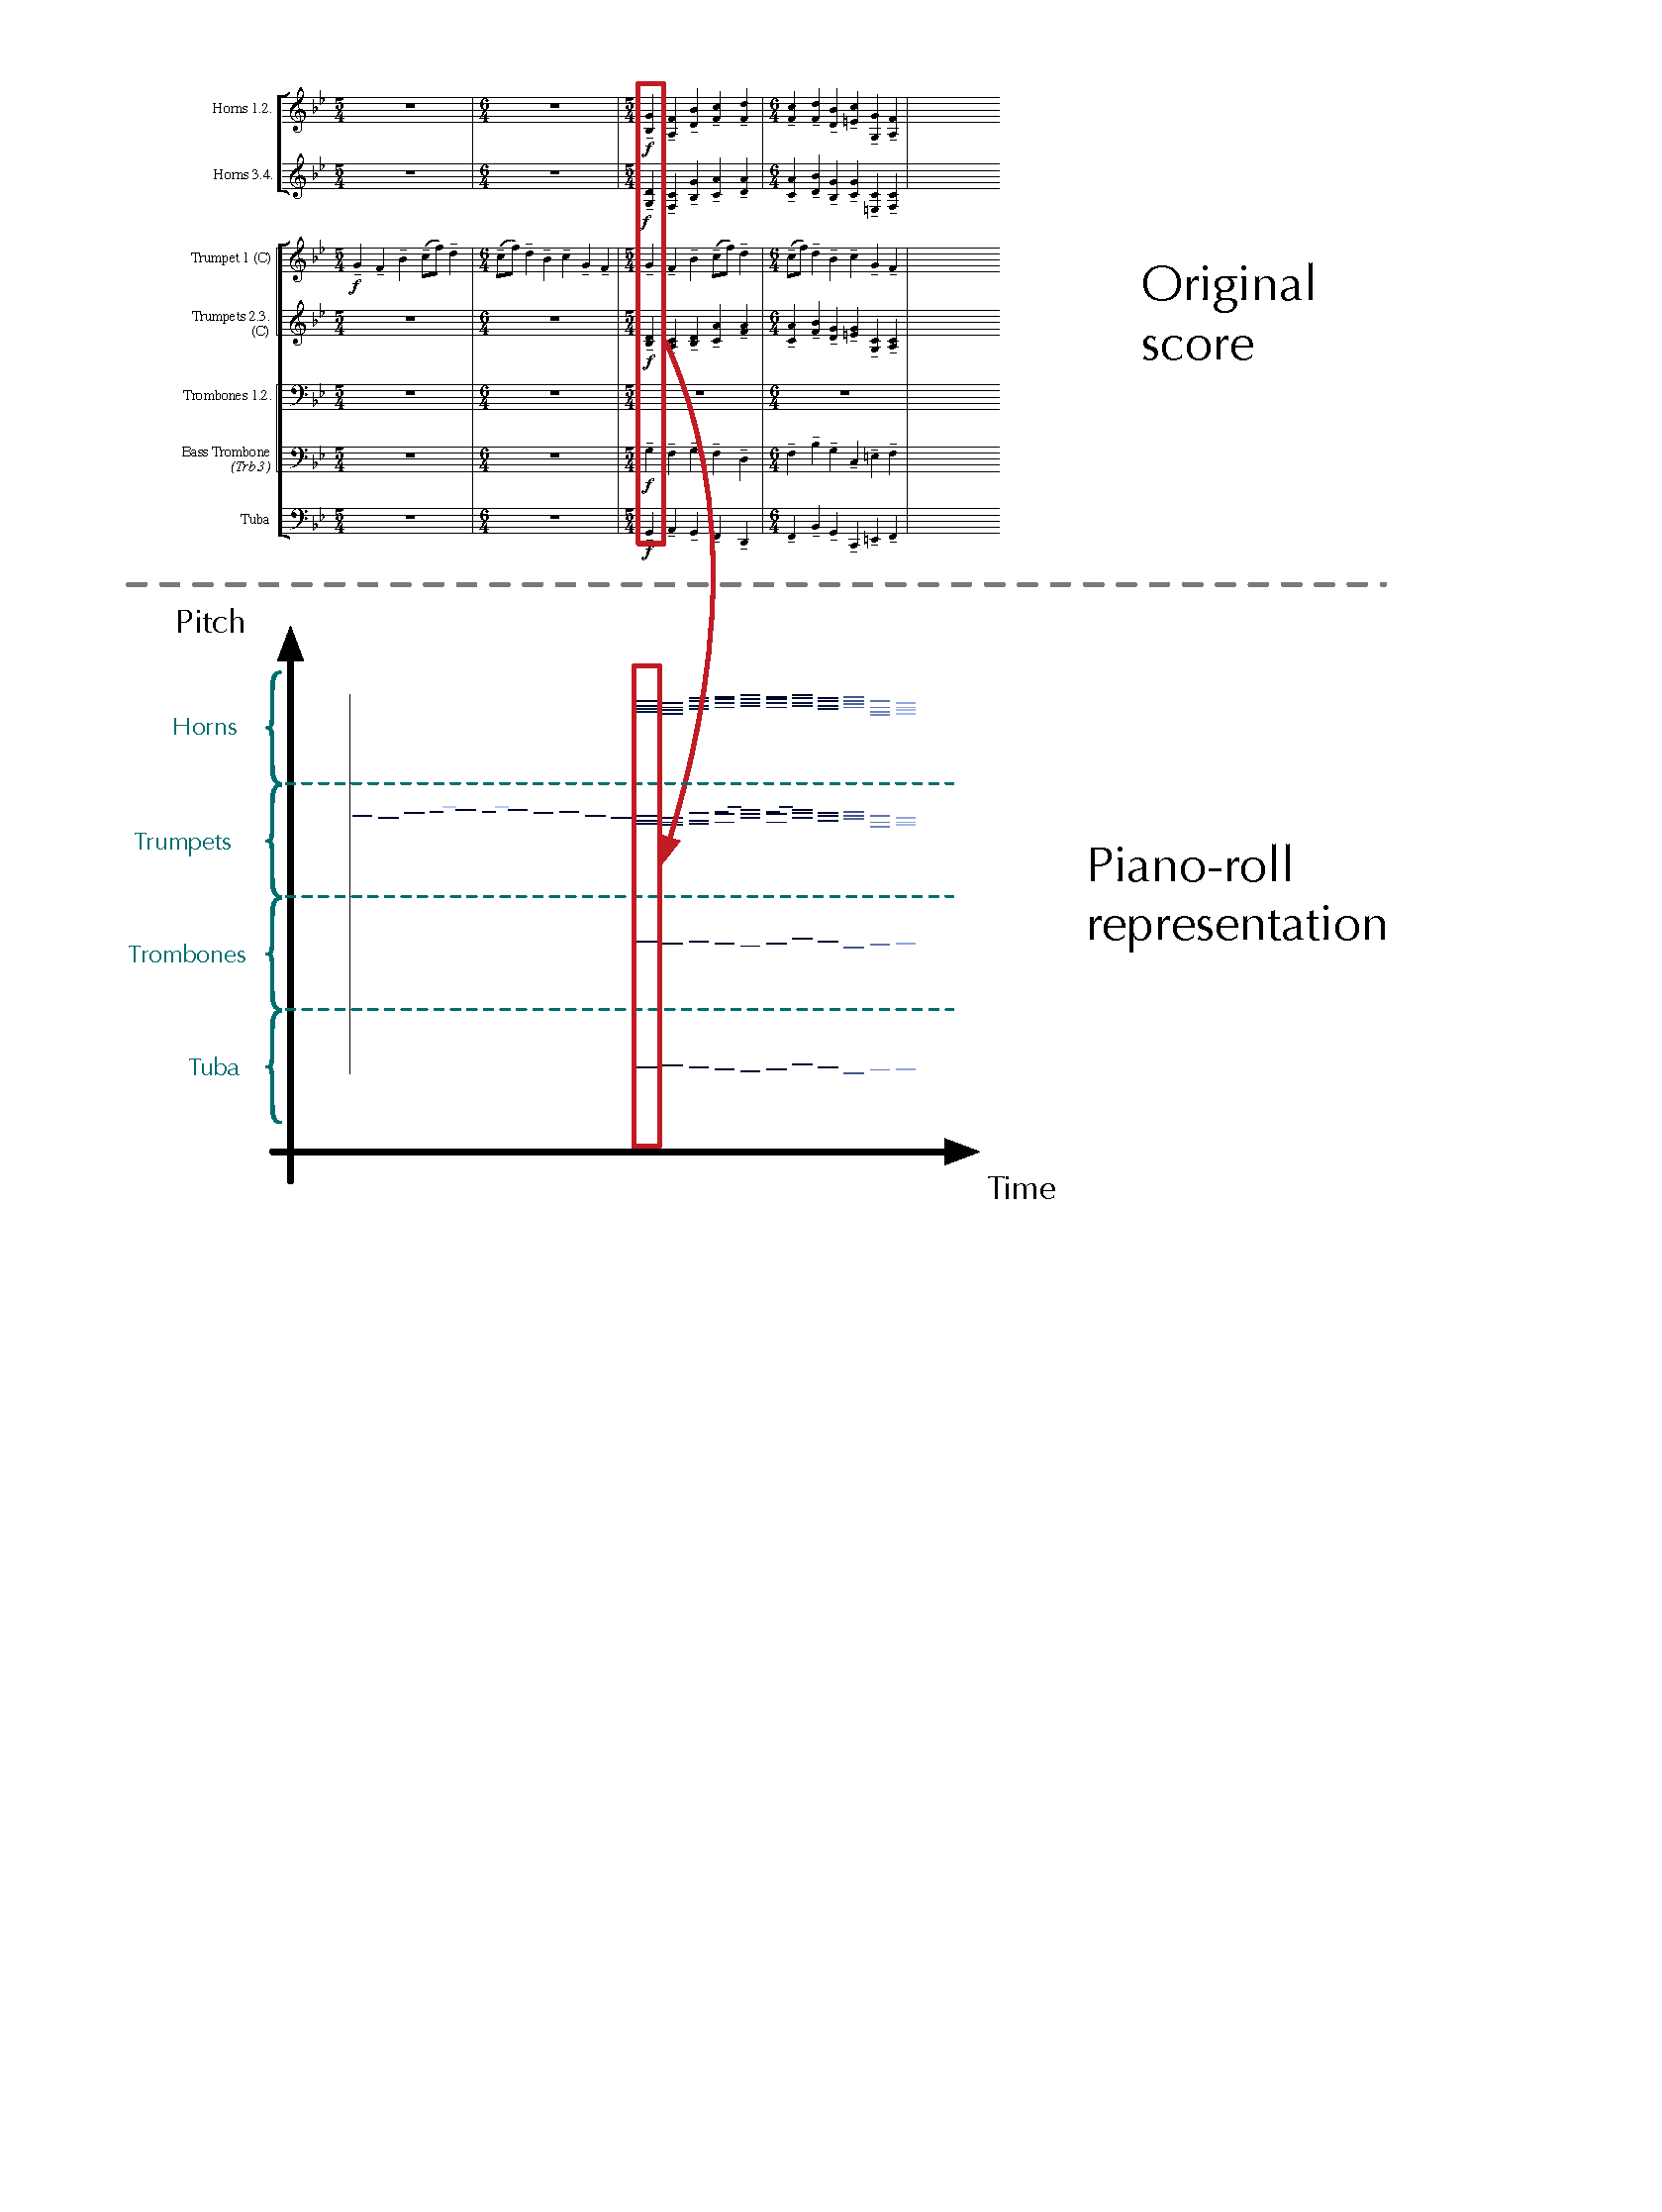
\includegraphics[scale=0.35]{Data_representation/from_score_to_pianoroll}
\caption{From the score of an orchestral piece, a convenient representation for computer processing named \textit{piano-roll} is extracted. A piano-roll $pr$ is a matrix whose rows represent pitches and columns represent a time frame depending on the discretization of time. A pitch $p$ at time $t$ played with an intensity $i$ is represented by $pr(p,t) = i$, $0$ being a note off. This definition is extended to an orchestra by simply concatenating the \textit{piano-rolls} of every instruments along the pitch dimension.}
\label{fig:piano-roll}
\end{figure}

% Aligner une séquence : on sait faire = Needleman
% Description Needleman-Wunsch
The \textit{Needleman-Wunsch}  algorithm \cite{NEEDLEMAN1970443} is a dynamic programming technique, which allows to find the optimal alignment of any two symbolic sequences, using only the introduction of gaps (\textit{i.e.} empty slots) in the sequences. Since we do not want to introduce silences in the scores, we remove section corresponding to empty slots for one of the file \textbf{SCHEMA MAIS CA VA ETRE GRAVE PETE COUILLE A FAIRE.}
The only requirement of this algorithm is to be able to define a scoring system, composed by a similarity function and a gap penalty. In our case defining a similarity function boils down to building a similarity measure between two vectors of a piano-roll.

% Similarity matrix
\paragraph{Similarity function}
To measure the similarity between two chords, we propose the following process :
\begin{itemize}
\item discard intensities : 1 represents a note being played, 0 a note off.
\item compute the pitch-class representation of the two vectors. A pitch-class is a set of all pitches that are a whole number of octave apart. 
In our case, we set a pitch-class to one if there is at least one note of the class that is played.
For instance, in our case, we set the pitch-class of C to 1 if there is one note with pitch C played in the chord.
It can be seen as an extremely rough approximation of the harmony.
After this step, two vectors of size 12 are obtained.
\item if one of the vector is only filled with zero, it represents a silence, and the similarity is automatically set to zero (note that the score can be negative).
\item else, for two pitch-class vectors A and B, we define the score as 
\begin{equation}
S \ = \ 5 \ \times \ \frac{\sum_{i=1}^{12} \delta(A_i , B_i)}{0.5 \ max(||A+B||_1 , 1)}
\label{eq:score_function}
\end{equation}
with
\[\delta(x) =
    \begin{cases*}
      0 & if x = 0\\
      -1 & if x = 1\\
      1 & if x = 2
    \end{cases*} 
\]
Note that the scaling factor 5 in the equation \prettyref{eq:score_function} has been set empirically. However, modifying its value can be compensated by the tuning parameters of the algorithm introduced in the next section.
\end{itemize}


\paragraph{Tuning the algorithm}
% Parameters
In addition to defining a score function, the \textit{Needleman-Wunsch} algorithm has to be carefully tuned by two parameters
\begin{itemize}
\item the gap open penalty defines the cost of introducing a gap in one of the two sequence
\item the gap extend penalty defines the cost of extending a gap in one of the two sequence
\end{itemize}
% Determining the parameters : grid-search
\textbf{The value of those parameters have been set by running a grid-search. Instead of the cumulative scores of the two aligned sequences, which depends on the value of the gap open and gap extend parameters, we used the number of 
CA C'EST LA MERDE : COMMENT CHOISIR UNE BONNE MESURE QUI DÉPEND PAS DES PARAMETRES ?}

\section{A case study : projective automatic orchestration}

In this section, we introduce and formalize the automatic projective orchestration task (\prettyref{fig:orch}). In particular, we propose a system based on statistical learning and define an evaluation framework that both rely on the \textbf{POD} database.

\subsection{Task definition}
\paragraph{Data representation}
In order to process the scores, we import them as \textit{piano-roll} matrices (see \prettyref{fig:piano-roll}). 
Its extension to represent an orchestra is straightforwardly obtained by the concatenation of the \textit{piano-rolls} of each instrument along the pitch dimension.

The rhythmic quantization is defined as the number of time frame in the \textit{piano-roll} per quarter note. When constructing the piano-rolls, we used a rhythmic quantization of 4.

In order to reduce the number of units, we systematically remove, for each instrument, any pitch which is never played in the training database. Hence, the dimension of the orchestral vector decreased from 2432 to 456 and the piano vector dimension from 128 to 88.
Also, we follow the classic orchestral simplifications used when writing orchestral scores by grouping together all the instruments of the same section. For instance, the \textit{violin} section, which might be composed by several instrumentalists, is written as a single part.
Finally, the velocity information is discarded, since we use binary units which solely indicate if a note is on or off.

\paragraph{Orchestral inference}
For each orchestral piece, we define $O(t)$ and $P(t)$ as the sequence of column vectors from the \textit{piano-roll} of the orchestra and piano part respectively, with $t \in \left[ 1,N_{T} \right]$ where $N_{T}$ is the length of the piano-roll, given a particular quantization.

At each time index $t$, the objective is to design a function that is able to infer the present orchestral frame knowing the recent past of the orchestra sequence and both past and present of the piano sequence. Mathematically, it consists in designing a function $f$ as
\begin{equation}
\begin{aligned}
\hat{O}(t) = \bm{f}\lbrack & O(t-1), ..., O(t-N), & \\
	& P(t), ... ,P(t-N) \rbrack & \forall t \in \left\lbrack|1, ... N_{T}|\right\rbrack\\
\end{aligned}
\label{eq:inference_function}
\end{equation}
$N$ defines the order of the model, and can freely be set.

\paragraph{Evaluation framework}
We propose an \textit{event-level orchestral inference} task to compare the performances of different models. \textbf{To our best knowledge, this is the first attempt to define a quantitative evaluation framework for automatic projective orchestration. USELESS ? + FAUX AU MOMENT OU ON PUBLIERA}

% Méthode générale
The proposed evaluation process first consists in extracting a subset of files in the database. We refer to this sub set as the \textit{test subset}. Then, for each file of this subset and for a given time index $t > N$, where N is the order of the model, the output $\hat{O}(t)$ given by \prettyref{eq:inference_function} can be compared to the ground-truth $O(t)$ read in the file.

% Comment comparer deux instants
To compare the inferred and ground-truth frames at time $t$, the accuracy measure commonly used in the music generation field \cite{DBLP:journals/corr/YaoCVDD15,boulanger2012modeling,lavrenko2003polyphonic} seems to be a good candidate. It is defined as
\begin{equation}
\text{Accuracy}(t)  = \frac{TP(t)}{TP(t) + FP(t) + FN(t)}
\label{eq:accuracy}
\end{equation}
where $TP(t)$ (true positives) is the number of notes correctly predicted (note played in both $\hat{O}(t)$ and $O(t)$). $FP(t)$ (false positive) is the number of notes predicted which are not in the original sequence (note played in $\hat{O}(t)$ but not in $O(t)$). $FN(t)$ (false negative) is the number on unreported notes (note absent in $\hat{O}(t)$, but played in $O(t)$). 
Note that in many other prediction framework, the true negatives also appears in the numerator and denominator of the accuracy measure. Because of the sparsity of the piano-roll representation, the accuracy values are squashed to 1 in most symbolic musical applications. Hence, the true negatives are not taken into consideration in the definition of the accuracy measure.

% Event level
Traditionally, in the music generation field, the accuracy measure is computed for each time frame $N <= t <= T_{N}$. However, it appears that a model which simply repeats the previous frame gradually becomes the best model as the quantization gets finer. Actually, this is already observed for a quantization of 4.
Hence, we suggest to compute the accuracy measure only for time indexes in $T_e$, the set of indexes $t_e$ such that
\[\text{Orch}(t_{e}) \neq \text{Orch}(t_{e} - 1)\]
Moreover, in the projective orchestration framework, rhythmic patterns are already established by the known piano score and, thus, does not have to be learned by the model.

% Au final, on mean simplement les différents score obtenus sur chaque event
Eventually, the mean accuracy measure over the dataset is given by
\begin{equation}
\frac{1}{K} \sum_{s \in \mathcal{D}_{test}} \sum_{t_e \in T_e(s)} Accuracy(t_e)
\end{equation}
where $\mathcal{D}_{test}$ define the test subset, $T_{e}(s)$ the set of event time indexes for the file s, and $K = \sum_{s \in \mathcal{D}_{test}} |T_e(s)|$

% Warning, if the design of the function is done by training, be careful with train/validate/test dataset
Note that in the case when the orchestral inference function is designed through a learning algorithm, the set of files used for the training step must carefully be kept disjoint from the test subset \cite{bishop2006pattern}.

\subsection{Proposed model}
We proposed a learning based approach, and developed N models. Their detailed description can be found in this article \textbf{REFFERRENEDCOSIDJPSDOC}.
The models we explored are defined in a probabilistic framework, were the vectors $O(t)$ and $P(t)$ are represented as random variables. The orchestral inference function takes the form of a neural network which expresses the conditional dependencies between the different variables (past, and present, orchestra and piano). The likelihood is used as a training objective.

\subsection{Results}
Four models are evaluated on the orchestral inference task. The first model is a random generation of the orchestral frames from a Bernoulli distribution of parameter $0.5$. The second model predicts an orchestral frame at time $t$ by repeating the frame at time $t-1$. Those two naive models constitute a first baseline against which we compare the cRBM and FGcRBM models.

The results are summed up in \prettyref{tab:result_event_level}. As expected, the random model has poor results. The repeat model performs significantly better. Indeed, it is relatively common that a note is sustained between two successive events. The cRBM largely outperforms those two models. However, the FGcRBM model has a lower score than the repeat model. We observed that the activation function of the visible units during the generative step was extremely noisy, which suggests that the training procedure mostly failed. We believe that this is due to the number of parameter,  and especially the dimension of the feature units. Indeed, in \cite{taylor2009factored}, only ten different configuration of the feature units were possible. When training on an orchestral database,  each different piano frame define a different configuration.

\begin{table}[h]
\centering
\begin{tabular}{c c}
\hline
Model & Orchestral Event-level (\%)\\
\hline
Random & 0.5\\ 
Repeat & 12.6\\
\hline \hline
cRBM & 23.2\\ 
FGcRBM & 6.2\\ 
\end{tabular}
\caption{Event-level accuracy for the orchestral inference task. Even though the cRBM performances increase by a factor 3 between the cRBM and the random model, the inclusion of features units provides a leap in the accuracy by multiplying the performances by 4.}
\label{tab:result_event_level}
\end{table}

\subsection{Limits of this framework}
% Limits of this task
% Ground-truth is not only truth

\section{Conclusion and future works}

\bibliographystyle{plain}
\bibliography{../Biblio/biblio}

%----------------------------------------------------------------------------------------

\end{document}
